\chapter{Systembeskrivelse}
Som før nævnt er systemet et automatisk vandingssystem. På figur \ref{photo:RigeBillede} ses et rigebillede af systemet. Systemet tilgås af et grafisk brugerinterface som vil være en webside der logges ind på via en PC. Her gives der mulighed for at se pH-værdi i karet, se hvor meget vand der er i karet, samt jordfugtigheden i gromedie. Der vil også være mulighed for at indstille disse værdier således systemet selv opretholder dem. Systemet er bestående af en  Raspberry-Pi som kører Raspbian, hvilket er en distribution af linux. Systemet kan måle fugtigheden i gromediet via en jordfugt-måler der kommunikerer via I2C.\newline 
Hvis fugtigheden når ned under et bestemt niveau tændes der for vandingen. I vandkaret er der iblandet gødning og en korrekt pH-værdi vil opretholdes af systemet. Systemet kan måle pH-værdien via en pH-probe som sidder fastmonteret i vandkaret.
 
\begin{figure}[H]
	\centering
	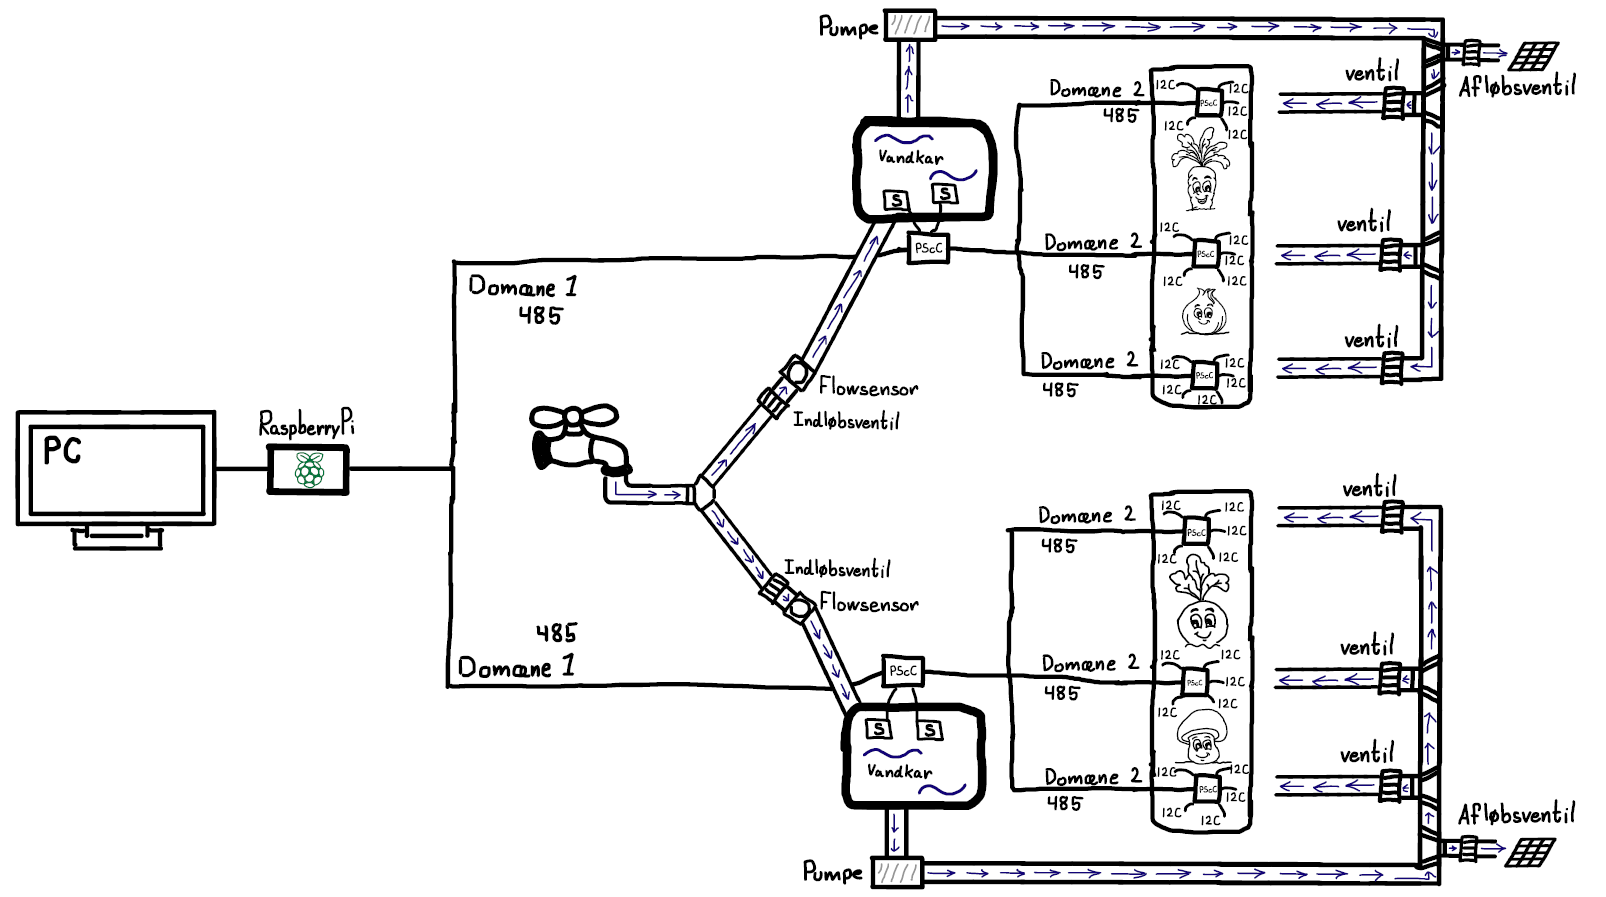
\includegraphics[scale=0.45]{Systembeskrivelse/rigebillede}
	\caption{Rigebillede af AVS}
	\label{photo:RigeBillede}
\end{figure}

Når systemet startes op vil vandkaret være tomt. For at fylde karet med vand, tændes der for indløbsventilen der sidder direkte i forlængelse af en vandhane. Hermed vil der løbe vand ned i karet og mængden måles vha.. flowsensor. Når der er løbet den ønskede mængde vand i karet, vil ventilen lukke og der vil automatisk blive doseret gødning indtil til en forudbestemt pH-værdi er nået. Skulle det ske, under opfyldning af det ikke lykkedes at lukke indløbsventilen vil der blive åbnet for afløbsventilen for at bibeholde et ønsket vandniveau.

Der er to aktører som kan tilgå systemet. Den ene er Brugeren, som tildaglig benytter systemet. Den anden er Teknikeren som tilgår systemet ved oprettelse, vedligeholdelse, samt nedlæggelse af systemet.\newline 
Systemetoprettelse sker i forhold til use casen "Opret kar", se Projektdokumenationen, afsnit 1.2. Herefter kan oprettes et ønsket antal sensorØ'er, her benyttes "Opret SensorØ"-usecasen. Når karet er oprettet skal pH-proben kalibreres via use casen "Kalibrer pH-probe", dette skal, som minimun gøres en gang hver måned for at kunne sikre en korrekt måling, dog gøres det også ved hver system-startup.\newline 
Styringen til vandkaret er implementeret på et "karPrint" her er pH-proben ligeledes koblet til. På printet, vil der være en rød LED som lyser når pH-proben skal kalibreres. Ved kalibrering sættes proben ned i en buffer-væske som har pH-værdien 7 og der trykkes på en knap på karprintet. KarControl vil herefter indlæse værdien og den røde LED skifter til en grøn. Karet kan også fyldes manuelt via use casen "Fyld kar". Her gives der mulighed for at åbne indløbsventilen, og lukke den når den ønskede mængde vand er løbet til.\newline 
I use cas'en "Indtast pH-værdi" gives der mulighed for at indtaste en pH-værdi som systemet skal opretholde. Det samme gives der mulighed for i "Indtast volumen". I use cas'en "Aflæs målinger" går Brugeren ind og aflæser værdierne fra sensorerne hvis det ønskes at se hvad status er. Use cas'en "Manuel vanding" giver mulighed for at vande manuelt. Dette kan være ønskeligt hvis systemet har fejl ved sensorene. Use cas'en "Tøm kar" bruges til at tømme karet og "Slet kar" er for at nedlægge et oprettet kar.
